
\documentclass[letterpaper,hide notes,xcolor={table,svgnames},pdftex]{beamer}
\def\showexamples{t}


%\usepackage[svgnames]{xcolor}

%% Demo talk
%\documentclass[letterpaper,notes=show]{beamer}

\usecolortheme{crane}
\setbeamertemplate{navigation symbols}{}

\usetheme{MyPittsburgh}
%\usetheme{Frankfurt}

%\usepackage{tipa}

\usepackage{hyperref}
\usepackage{graphicx,xspace}
\usepackage[normalem]{ulem}

\newcommand\SF[1]{$\bigstar$\footnote{SF: #1}}



\newcounter{tmpnumSlide}
\newcounter{tmpnumNote}

% old question code
%\newcommand\question[1]{{$\bigstar$ \small \onlySlide{2}{#1}}}
% \newcommand\nquestion[1]{\ifdefined \presentationonly \textcircled{?} \fi \note{\par{\Large \textbf{?}} #1}}
% \newcommand\nanswer[1]{\note{\par{\Large \textbf{A}} #1}}


 \newcommand\mnote[1]{%
   \addtocounter{tmpnumSlide}{1}
   \ifdefined\showcues {~\tiny\fbox{\arabic{tmpnumSlide}}}\fi
   \note{\setlength{\parskip}{1ex}\addtocounter{tmpnumNote}{1}\textbf{\Large \arabic{tmpnumNote}:} {#1\par}}}

\newcommand\mmnote[1]{\note{\setlength{\parskip}{1ex}#1\par}}

%\newcommand\mnote[2][]{\ifdefined\handoutwithnotes {~\tiny\fbox{#1}}\fi
% \note{\setlength{\parskip}{1ex}\textbf{\Large #1:} #2\par}}

%\newcommand\mnote[2][]{{\tiny\fbox{#1}} \note{\setlength{\parskip}{1ex}\textbf{\Large #1:} #2\par}}

\newcommand\mquestion[2]{{~\color{red}\fbox{?}}\note{\setlength{\parskip}{1ex}\par{\Large \textbf{?}} #1} \note{\setlength{\parskip}{1ex}\par{\Large \textbf{A}} #2\par}\ifdefined \presentationonly \pause \fi}

\newcommand\blackboard[1]{%
\ifdefined   \showblackboard
  {#1}
  \else {\begin{center} \fbox{\colorbox{blue!30}{%
         \begin{minipage}{.95\linewidth}%
           \hspace{\stretch{1}} Some space intentionally left blank; done at the blackboard.%
         \end{minipage}}}\end{center}}%
         \fi%
}



%\newcommand\q{\tikz \node[thick,color=black,shape=circle]{?};}
%\newcommand\q{\ifdefined \presentationonly \textcircled{?} \fi}

\usepackage{listings}
\lstset{%
  keywordstyle=\bfseries,
  aboveskip=15pt,
  belowskip=15pt,
  captionpos=b,
  identifierstyle=\ttfamily,
  escapeinside={(*@}{@*)},
  stringstyle=\ttfamiliy,
  frame=lines,
  numbers=left, basicstyle=\scriptsize, numberstyle=\tiny, stepnumber=0, numbersep=2pt}

\usepackage{siunitx}
\newcommand\sius[1]{\num[group-separator = {,}]{#1}\si{\micro\second}}
\newcommand\sims[1]{\num[group-separator = {,}]{#1}\si{\milli\second}}
\newcommand\sins[1]{\num[group-separator = {,}]{#1}\si{\nano\second}}
\sisetup{group-separator = {,}, group-digits = true}

%% -------------------- tikz --------------------
\usepackage{tikz}
\usetikzlibrary{positioning}
\usetikzlibrary{arrows,backgrounds,automata,decorations.shapes,decorations.pathmorphing,decorations.markings,decorations.text}

\tikzstyle{place}=[circle,draw=blue!50,fill=blue!20,thick, inner sep=0pt,minimum size=6mm]
\tikzstyle{transition}=[rectangle,draw=black!50,fill=black!20,thick, inner sep=0pt,minimum size=4mm]

\tikzstyle{block}=[rectangle,draw=black, thick, inner sep=5pt]
\tikzstyle{bullet}=[circle,draw=black, fill=black, thin, inner sep=2pt]

\tikzstyle{pre}=[<-,shorten <=1pt,>=stealth',semithick]
\tikzstyle{post}=[->,shorten >=1pt,>=stealth',semithick]
\tikzstyle{bi}=[<->,shorten >=1pt,shorten <=1pt, >=stealth',semithick]

\tikzstyle{mut}=[-,>=stealth',semithick]

\tikzstyle{treereset}=[dashed,->, shorten >=1pt,>=stealth',thin]

\usepackage{ifmtarg}
\usepackage{xifthen}
\makeatletter
% new counter to now which frame it is within the sequence
\newcounter{multiframecounter}
% initialize buffer for previously used frame title
\gdef\lastframetitle{\textit{undefined}}
% new environment for a multi-frame
\newenvironment{multiframe}[1][]{%
\ifthenelse{\isempty{#1}}{%
% if no frame title was set via optional parameter,
% only increase sequence counter by 1
\addtocounter{multiframecounter}{1}%
}{%
% new frame title has been provided, thus
% reset sequence counter to 1 and buffer frame title for later use
\setcounter{multiframecounter}{1}%
\gdef\lastframetitle{#1}%
}%
% start conventional frame environment and
% automatically set frame title followed by sequence counter
\begin{frame}%
\frametitle{\lastframetitle~{\normalfont(\arabic{multiframecounter})}}%
}{%
\end{frame}%
}
\makeatother

\makeatletter
\newdimen\tu@tmpa%
\newdimen\ydiffl%
\newdimen\xdiffl%
\newcommand\ydiff[2]{%
    \coordinate (tmpnamea) at (#1);%
    \coordinate (tmpnameb) at (#2);%
    \pgfextracty{\tu@tmpa}{\pgfpointanchor{tmpnamea}{center}}%
    \pgfextracty{\ydiffl}{\pgfpointanchor{tmpnameb}{center}}%
    \advance\ydiffl by -\tu@tmpa%
}
\newcommand\xdiff[2]{%
    \coordinate (tmpnamea) at (#1);%
    \coordinate (tmpnameb) at (#2);%
    \pgfextractx{\tu@tmpa}{\pgfpointanchor{tmpnamea}{center}}%
    \pgfextractx{\xdiffl}{\pgfpointanchor{tmpnameb}{center}}%
    \advance\xdiffl by -\tu@tmpa%
}
\makeatother
\newcommand{\copyrightbox}[3][r]{%
\begin{tikzpicture}%
\node[inner sep=0pt,minimum size=2em](ciimage){#2};
\usefont{OT1}{phv}{n}{n}\fontsize{4}{4}\selectfont
\ydiff{ciimage.south}{ciimage.north}
\xdiff{ciimage.west}{ciimage.east}
\ifthenelse{\equal{#1}{r}}{%
\node[inner sep=0pt,right=1ex of ciimage.south east,anchor=north west,rotate=90]%
{\raggedleft\color{black!50}\parbox{\the\ydiffl}{\raggedright{}#3}};%
}{%
\ifthenelse{\equal{#1}{l}}{%
\node[inner sep=0pt,right=1ex of ciimage.south west,anchor=south west,rotate=90]%
{\raggedleft\color{black!50}\parbox{\the\ydiffl}{\raggedright{}#3}};%
}{%
\node[inner sep=0pt,below=1ex of ciimage.south west,anchor=north west]%
{\raggedleft\color{black!50}\parbox{\the\xdiffl}{\raggedright{}#3}};%
}
}
\end{tikzpicture}
}


%% --------------------

%\usepackage[excludeor]{everyhook}
%\PushPreHook{par}{\setbox0=\lastbox\llap{MUH}}\box0}

%\vspace*{\stretch{1}

%\setbox0=\lastbox \llap{\textbullet\enskip}\box0}

\setlength{\parskip}{\fill}

\newcommand\noskips{\setlength{\parskip}{1ex}}
\newcommand\doskips{\setlength{\parskip}{\fill}}

\newcommand\xx{\par\vspace*{\stretch{1}}\par}
\newcommand\xxs{\par\vspace*{2ex}\par}
\newcommand\tuple[1]{\langle #1 \rangle}
\newcommand\code[1]{{\sf \footnotesize #1}}
\newcommand\ex[1]{\uline{Example:} \ifdefined \presentationonly \pause \fi
  \ifdefined\showexamples#1\xspace\else{\uline{\hspace*{2cm}}}\fi}

\newcommand\ceil[1]{\lceil #1 \rceil}


\AtBeginSection[]
{
   \begin{frame}
       \frametitle{Outline}
       \tableofcontents[currentsection]
   \end{frame}
}



\pgfdeclarelayer{edgelayer}
\pgfdeclarelayer{nodelayer}
\pgfsetlayers{edgelayer,nodelayer,main}

\tikzstyle{none}=[inner sep=0pt]
\tikzstyle{rn}=[circle,fill=Red,draw=Black,line width=0.8 pt]
\tikzstyle{gn}=[circle,fill=Lime,draw=Black,line width=0.8 pt]
\tikzstyle{yn}=[circle,fill=Yellow,draw=Black,line width=0.8 pt]
\tikzstyle{empty}=[circle,fill=White,draw=Black]
\tikzstyle{bw} = [rectangle, draw, fill=blue!20, 
    text width=4em, text centered, rounded corners, minimum height=2em]
    
    \newcommand{\CcNote}[1]{% longname
	This work is licensed under the \textit{Creative Commons #1 3.0 License}.%
}
\newcommand{\CcImageBy}[1]{%
	\includegraphics[scale=#1]{creative_commons/cc_by_30.pdf}%
}
\newcommand{\CcImageSa}[1]{%
	\includegraphics[scale=#1]{creative_commons/cc_sa_30.pdf}%
}
\newcommand{\CcImageNc}[1]{%
	\includegraphics[scale=#1]{creative_commons/cc_nc_30.pdf}%
}
\newcommand{\CcGroupBySa}[2]{% zoom, gap
	\CcImageBy{#1}\hspace*{#2}\CcImageNc{#1}\hspace*{#2}\CcImageSa{#1}%
}
\newcommand{\CcLongnameByNcSa}{Attribution-NonCommercial-ShareAlike}

\newenvironment{changemargin}[1]{% 
  \begin{list}{}{% 
    \setlength{\topsep}{0pt}% 
    \setlength{\leftmargin}{#1}% 
    \setlength{\rightmargin}{1em}
    \setlength{\listparindent}{\parindent}% 
    \setlength{\itemindent}{\parindent}% 
    \setlength{\parsep}{\parskip}% 
  }% 
  \item[]}{\end{list}} 




\title{Lecture 28 --- Interval \& Watchdog Timers}

\author{Patrick Lam \& Jeff Zarnett\\ \small \texttt{p.lam@ece.uwaterloo.ca} \& \texttt{jzarnett@uwaterloo.ca}}
\institute{Department of Electrical and Computer Engineering \\
  University of Waterloo}
\date{\today}

\begin{document}

\begin{frame}
  \titlepage
\end{frame}


\begin{frame}
\frametitle{Concept: Timers in Embedded Systems}

\begin{changemargin}{1cm}
\large

Today: How to use timers,\\ \qquad \qquad e.g. in embedded~systems:
\begin{itemize}
\item Interval Timers
\item Watchdog Timers
\end{itemize}
~\\
We'll use Java timers to implement these,
and learn the difference between Android and Java timers.

\end{changemargin}

\end{frame}

\begin{frame}
\frametitle{Applications of Timers}

\Large
\begin{changemargin}{1.3cm}
Interval Timers---perform a task occasionally.\\[-0.5em]
\begin{itemize}\item (raising alarms; polling).
\end{itemize}
~\\
Watchdog Timers---reset a stuck system.
~\\[1em]

\end{changemargin}

\end{frame}

\part{Interval Timers}
\frame{\partpage}

\begin{frame}
\frametitle{Interval Timers}

\begin{changemargin}{1cm}
\large

Good for recurring tasks.\\[1em]

Example: Light sensor polling\\
 (but not on Android---receive sensor events instead).\\[1em]

Previously: {\tt Handler} for interval timers.

\end{changemargin}

\end{frame}

\begin{frame}[fragile]
\frametitle{Handlers for Infinitely-Recurring Interval Timers}

\begin{lstlisting}
  Handler h = new Handler();
  Runnable r = new Runnable() {
    public void run() {
      // execute the task
      h.postDelayed(this, delayInMS);
    }
  };
  h.postDelayed(r, delayInMS);
\end{lstlisting}

\end{frame}

\begin{frame}[fragile]
\frametitle{Cancelling Tasks}

\begin{changemargin}{1cm}
By the way, you can cancel an upcoming task like this:
\begin{lstlisting}
  h.removeCallbacks(r);
\end{lstlisting}
\end{changemargin}
\end{frame}

\begin{frame}
\frametitle{True Interval Timers}

\large
\begin{changemargin}{1cm}
Handlers run when the thread is available.\\[1em]

True interval timers interrupt the processor.

Can simulate with {\tt java.util.Timer}\footnote{\url{http://steve.odyfamily.com/?p=12}, accessed
  February 3, 2013.}. \\[1em]

Payload runs in a different thread:
\begin{itemize}
\item[(+)] more predictable timing;
\item[(--)] can't update UI from other thread.
\end{itemize}
~\\
Generally more overhead for {\tt java.util.Timer}, not great for Android apps.
\end{changemargin}
\end{frame}

\begin{frame}[fragile]
\frametitle{Getting Around UI Thread Issues}

\begin{changemargin}{1cm}
Start the Timer like this:

\begin{lstlisting}
  Timer t = new Timer();
  t.schedule(new TimerTask() {
    @Override
    public void run() {
      runOnUiThread(timerTick);
    }
  }, firstDelayMS, repeatIntervalMS);
\end{lstlisting}
If you omit repeatIntervalMS, you get a one-shot timer.

Don't call {\tt timerTick.run()} directly.
\end{changemargin}

\end{frame}

\begin{frame}[fragile]
\frametitle{Programming timerTick}

\begin{changemargin}{1cm}
Put your UI-manipulating code in {\tt timerTick}:
\begin{lstlisting}
Runnable timerTick = new Runnable() {
  @Override
  public void run() {
    Toast.makeText(getApplicationContext(), 
                   "ding!", 
                   Toast.LENGTH_SHORT).show();
  }
};
\end{lstlisting}
\end{changemargin}

\end{frame}

\begin{frame}

\frametitle{Java Timer summary}

\begin{changemargin}{1cm}
\large
To use a Java Timer:
\begin{enumerate}
\item instantiate a new {\tt Timer} object;
\item schedule {\tt TimerTask} on that {\tt Timer};
\item inside the {\tt TimerTask}, invoke {\tt Runnable} to run on the
UI thread; and
\item implement the {\tt run()} method on the {\tt Runnable} to effect
  UI changes.  
\end{enumerate}
\end{changemargin}

\end{frame}

\part{Watchdog Timers}
\frame{\partpage}

\begin{frame}

\frametitle{Goal of a Watchdog Timer}

\Large
\begin{changemargin}{1cm}
Observe that a system appears to
be stuck and take some action.
\end{changemargin}

\end{frame}

\begin{frame}
\frametitle{About Watchdog Timers}
\begin{changemargin}{1cm}
Commonly found in computer systems where humans cannot easily take corrective action.

If a NASA satellite is stuck, it's hard to send astronauts up to push the reset button.

If not for the ability to automatically restart, the satellite could be permanently disabled.

\end{changemargin}
\end{frame}

\begin{frame}
\frametitle{About Watchdog Timers}
\begin{changemargin}{1cm}

The system needs to indicate, before the limit of the timer, that everything is okay. 

If the system thinks all is well, either by checking some fault conditions or simply by default, the watchdog timer is reset. 


\end{changemargin}
\end{frame}


\begin{frame}
\frametitle{Watchdog Example}
\begin{changemargin}{1cm}

Checking if free memory is below 256~MB. 

If the system detects free memory is $>$256~MB, reset timer.

If it is below 256~MB, then the watchdog timer is not reset. \\
\quad The timer will fire.

Corrective action takes place: (i.e., freeing up some memory).\mnote{Corrective action is variable, based on the system the watchdog is looking after. In some cases, corrective action is minor (killing a task), but in physical systems it might be necessary to turn off motors for safety. }


\end{changemargin}
\end{frame}



\begin{frame}

\frametitle{Implementing a Watchdog Timer}

\begin{changemargin}{1cm}
Can build a watchdog timer using an interval timer:
\begin{itemize}
\item Set the timer interval to be the largest allowable time for a task
to take. Start the timer.
\item If the timer fires, the task took too long.
\item The timer event handler deals with
the situation\\~~~~ (e.g. by killing the task.)
\end{itemize}
\end{changemargin}
\end{frame}


\begin{frame}
\frametitle{Resilience for Watchdog Timers}

\Large
\begin{changemargin}{1cm}
In an embedded system: \\~~~specialized~hardware.\\[1em]

Timer has some resilience: \\~~~runs in a separate thread.
\end{changemargin}

\end{frame}

\begin{frame}
\frametitle{Android Watchdog Timer}

\begin{changemargin}{1cm}
\large
Summary: 
\begin{itemize} 
\item start the watchdog timer;
\item the timer runs a task $t$ on the UI thread;
\item task $t$ kills the activity; and
\item set up a click listener to go to a web page instead.
\end{itemize}
\end{changemargin}
\end{frame}

\begin{frame}
\frametitle{Outcomes from Watchdog Timer}
\begin{changemargin}{1cm}
\Large
\begin{enumerate}
\item If you click the button soon enough, \\
~~~app goes to the web page;
\item Otherwise, the Activity finishes.
\end{enumerate}
\end{changemargin}
\end{frame}

\begin{frame}
\frametitle{Multiple Stage Watchdog Timers}
\begin{changemargin}{1cm}
So far corrective action has been all-or-nothing. 

We can have multiple stages -- multiple levels of response. 

If the first level of response does not resolve the problem: \\
\quad second level of response activates; takes more drastic action. 


\end{changemargin}
\end{frame}

\begin{frame}
\frametitle{Two Stage Watchdog Timer Example}
\begin{changemargin}{1cm}

The first watchdog timer attempts to restart \texttt{example.exe}. 

The first level has a timer length of 180 seconds; every 60 seconds, \texttt{example.exe} resets the watchdog timer. 

If the reset doesn't happen, the watchdog activates. 

Watchdog 1: starts watchdog 2, with a length of 120 seconds. Then the first watchdog tries to restart \texttt{example.exe}. 

If the first watchdog does not successfully restart the program within the 120 seconds, the second watchdog timer activates and restarts the computer.


\end{changemargin}
\end{frame}

\begin{frame}
\frametitle{Timer Coalescing}
\begin{changemargin}{1cm}

Using timers has an impact on power consumption. 

Suppose an interval timer set up with an interval of 1000ms. 

Every second the system will execute the timer's action -- the system wakes up, runs the action, then goes back to sleep. 

\end{changemargin}
\end{frame}

\begin{frame}
\frametitle{Timer Coalescing}
\begin{changemargin}{1cm}

What if there are multiple interval timers?

The system might never actually get to sleep; \\
\quad constantly being woken up by interval timers.

\end{changemargin}
\end{frame}

\begin{frame}
\frametitle{Timer Coalescing}
\begin{center}
	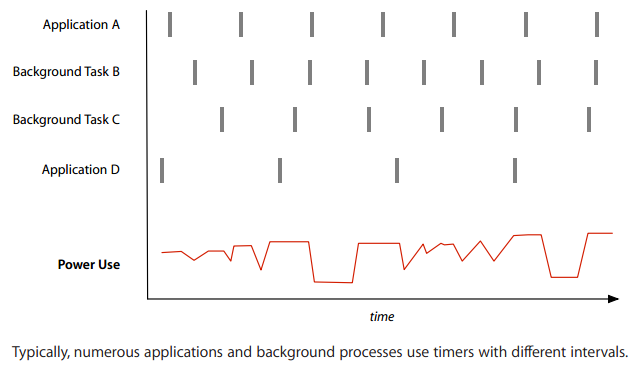
\includegraphics[width=0.85\textwidth]{images/coalesced_before.png}
\end{center}

\end{frame}

\begin{frame}
\frametitle{Timer Coalescing Semantics}
\begin{changemargin}{1cm}

A critical insight about timers. 

For a 1000ms timer, the system does not promise that the timer will run exactly 1000 ms from now. 

What it really says is that the timer task will execute \alert{no sooner than} 1000 ms from now. 

It could be 1004 ms or 1200 ms later;\\
\quad yet it could not be 997 ms or 980 ms later.


\end{changemargin}
\end{frame}

\begin{frame}
\frametitle{Timer Coalescing Semantics}
\begin{changemargin}{1cm}

The OS can do something clever using these semantics.

Delay some timers a little bit so that they line up.

\end{changemargin}
\end{frame}

\begin{frame}
\frametitle{Timer Coalescing}
\begin{center}
	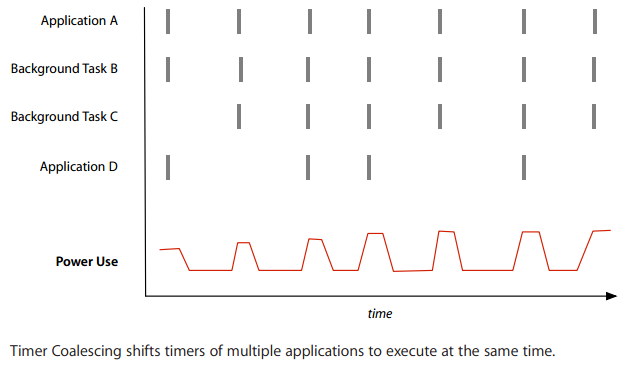
\includegraphics[width=0.85\textwidth]{images/coalesced-after.png}
\end{center}

\end{frame}


\begin{frame}
\frametitle{Timer Coalescing Semantics}
\begin{changemargin}{1cm}

Now, this image is not a hundred percent accurate. 

Some of the lines were moved to the left (back in time) to make them line up. \mnote{and that would violate the no-sooner-than semantics.}

This is just artistic license; in reality the lines could only be shifted to the right.

Most modern operating systems do this, including Windows and Mac OS X.

\end{changemargin}
\end{frame}


\end{document}
